\subsection{AHTR Moltres Temperature Model}
\begin{frame}
    \frametitle{AHTR Temperature Model}
    \begin{block}{AHTR Temperature Model}
        \begin{itemize}
            \item I used the open-source MSR simulation tool, Moltres, to conduct AHTR
            full assembly multiphysics simulations 
            \item AHTR Moltres simulations captures thermal feedback effects, absent
            from the purely neutronics OpenMC simulations
            \item I model the steady-state temperature of a 2D x-y AHTR cross-section
        \end{itemize}
    \end{block}
    \begin{block}{Assumptions}
        \begin{itemize}
            \item Conductive heat transfer 
            \item Heat removal by uniform salt flow in coolant regions
        \end{itemize}
    \end{block}

\end{frame}

\begin{frame}
    \frametitle{AHTR Temperature Model Setup}
    \begin{block}{Steps to produce Moltres AHTR Temperature Model}
        \begin{itemize}
          \item OpenMC neutronics model produces group constants data 
          \item Mesh generation
          \item Run Moltres model to calculate temperature distribution 
          (accepts group constants data and mesh)
        \end{itemize}
    \end{block}
    For successful AHTR Moltres simulation, I must establish suitable spatial and
    energy homogenization that preserves accuracy while maintaining an acceptable
    runtime
    \begin{block}{Energy Homogenization}
        \begin{table}[]
            \centering
            \begin{minipage}[c]{0.6\textwidth}
                \centering
                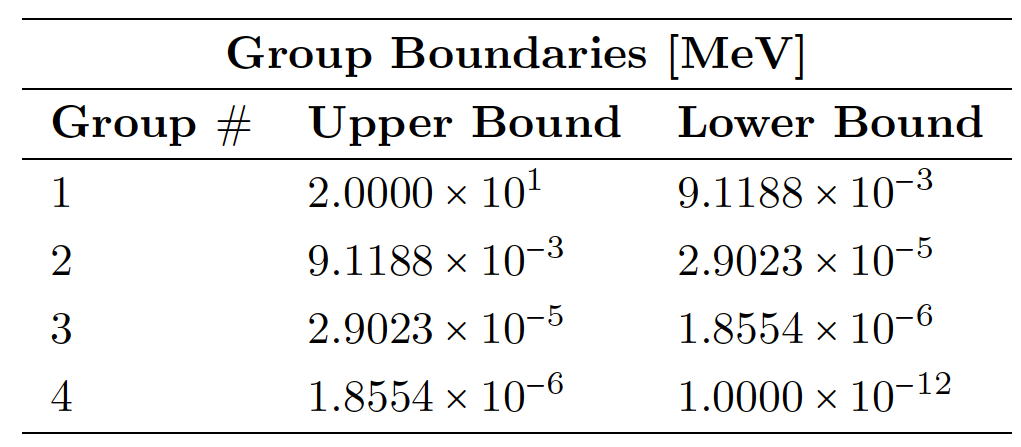
\includegraphics[width=0.8\linewidth]{figures/ahtr-energy-discr.png}
            \end{minipage}\hfill
            \begin{minipage}[c]{0.4\textwidth}
            \caption{4-group energy structures for AHTR geometry 
            derived by \cite{gentry_development_2016}.}
        \end{minipage}
        \end{table}
    \end{block}
\end{frame}

\begin{frame}
    \frametitle{AHTR Temperature Model Spatial Homogenization}
        \textbf{Fuel assembly 61 cell discretization}: inter-assembly FLiBe, 
        Y-shaped graphite structure, control rod slot FLiBe, graphite spacers, 
        each diamond shape section's inter-plank FLiBe (3), each graphite plank (18), 
        and each fuel stripe (36)
    \begin{figure}[]
            \centering
            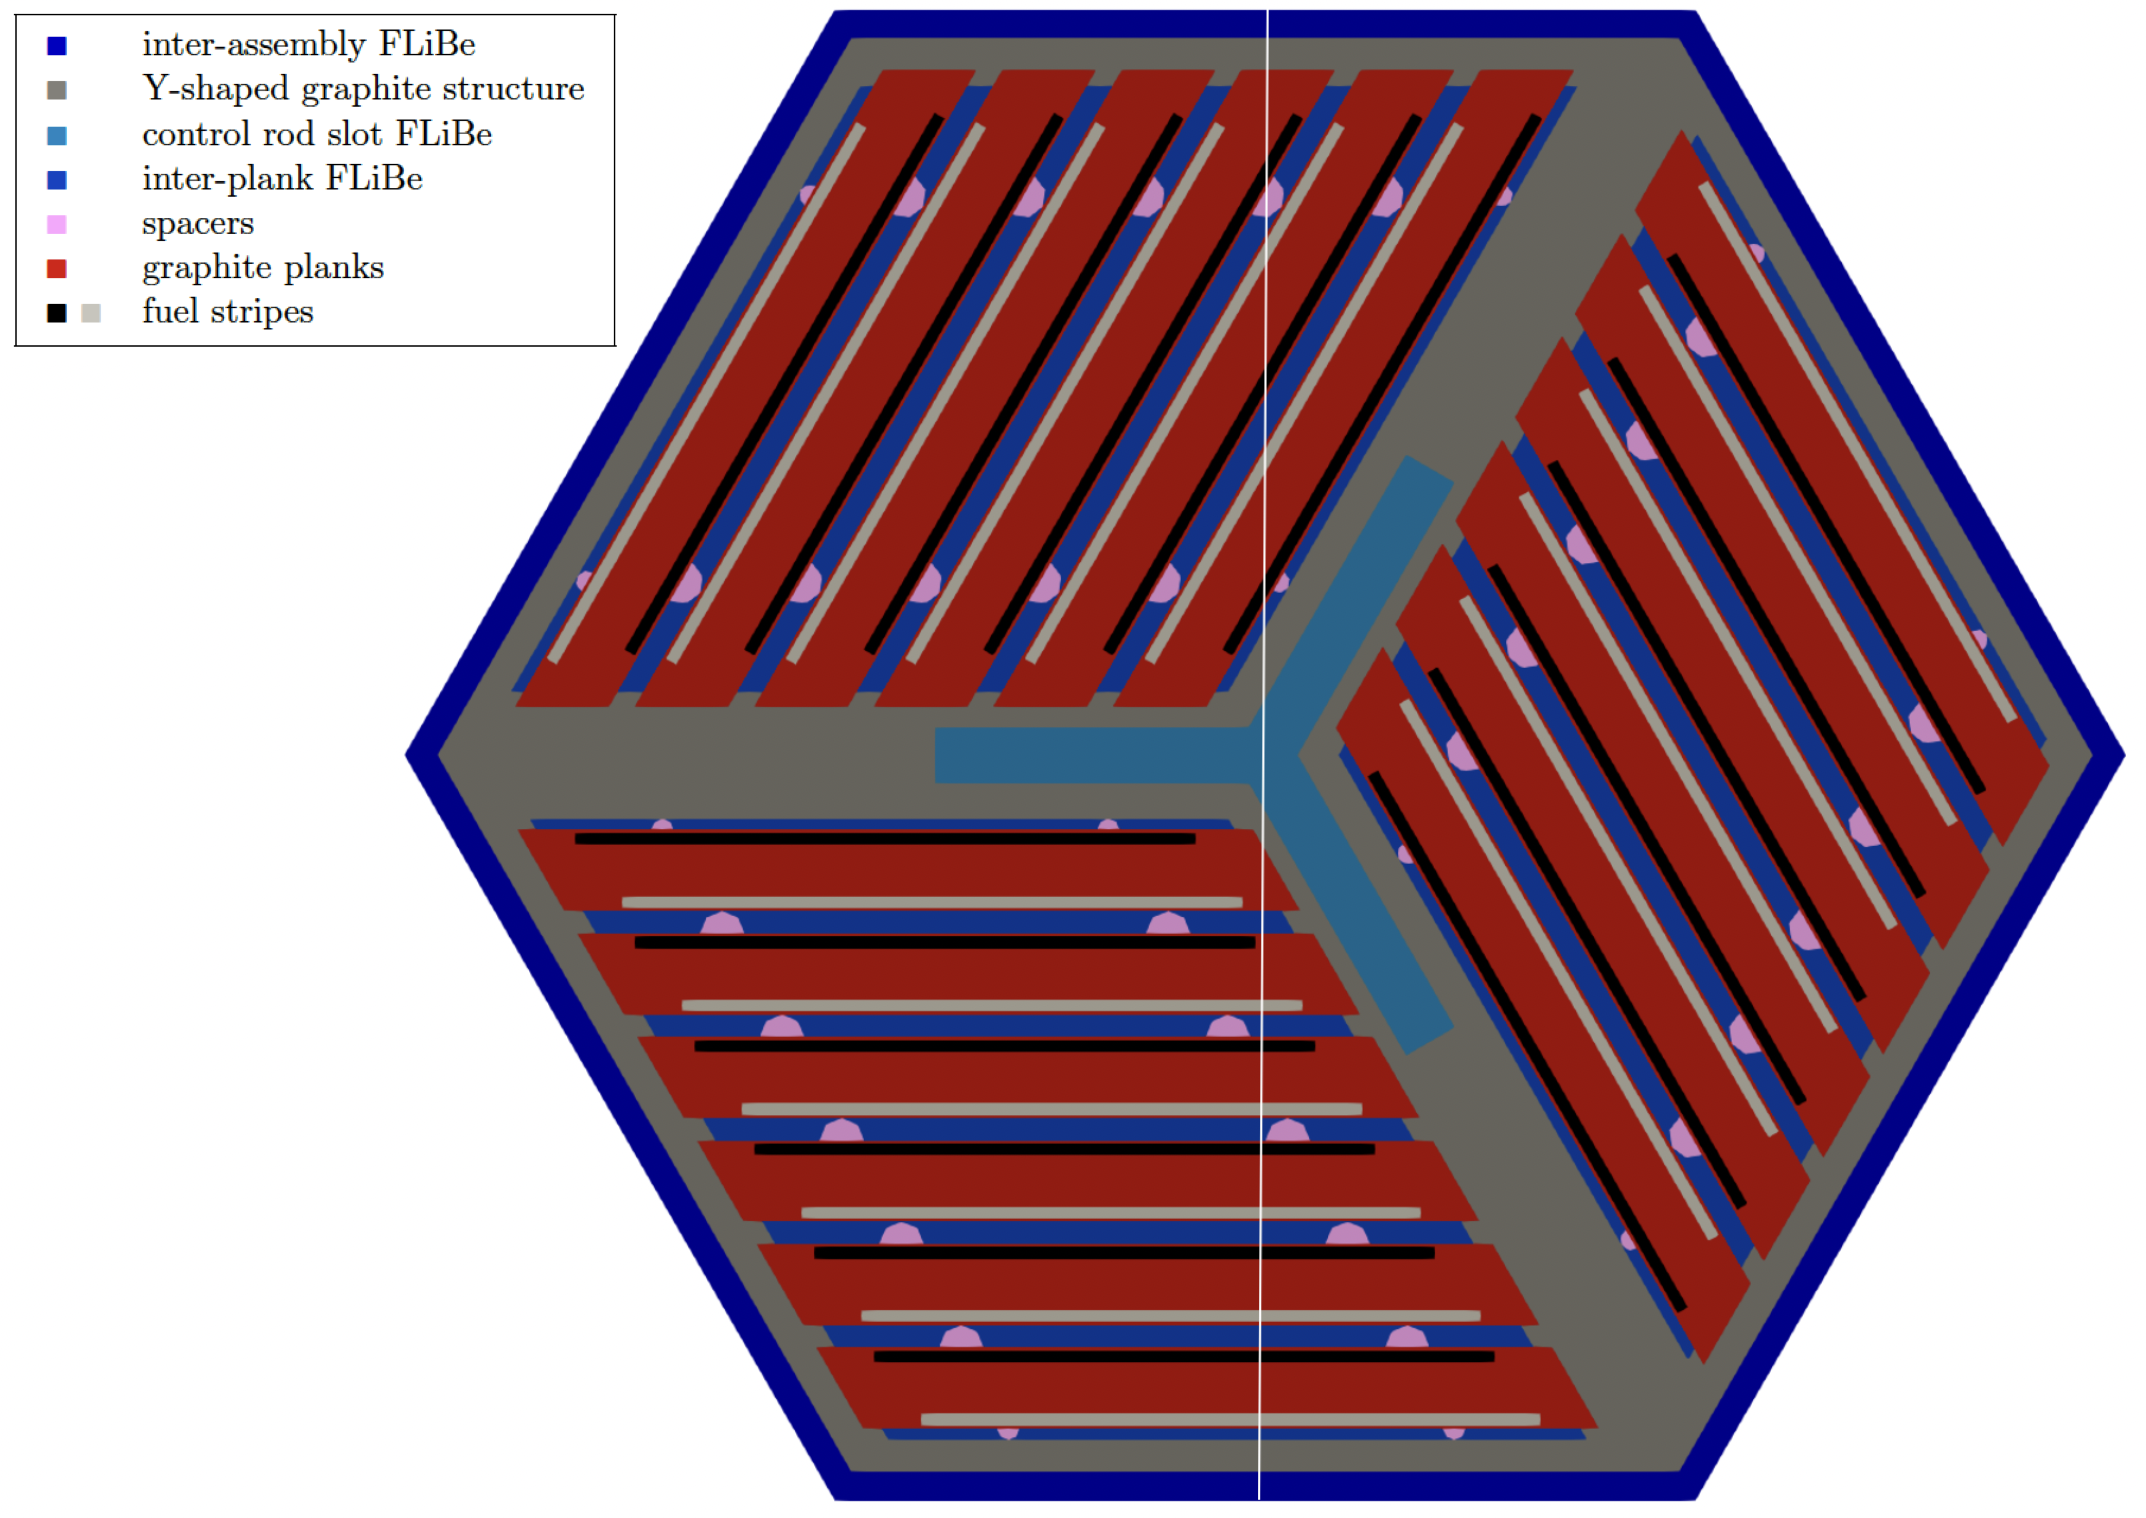
\includegraphics[width=0.65\linewidth]{figures/assembly_mg_pres.png}
        \caption{AHTR assembly spatial homogenization for group constant generation.}
    \end{figure}
\end{frame}

\subsection{Key Neutronics Parameters Verification}
\begin{frame}
    \frametitle{AHTR Temp Model Key Neutronics Parameter Verification}
    I \textbf{verify acceptable spatial homogenization and energy discretization} by 
    comparing key neutronics parameters (KNPs) between: 
    \begin{itemize} 
        \item OpenMC simulation with continuous energy and TRISO-level spatial fidelity
        \item Moltres simulation with 4-group energy and spatial homogenization
    \end{itemize}
    \textbf{KNPs}: $k_{eff}$, reactivity coefficients, flux distribution, and neutron 
    spectrum
    \begin{itemize}
        \item All comparisons are to verify that the Moltres model is replicating the 
        OpenMC model's neutronics correctly
    \end{itemize}
    \textbf{Reactivity coefficients and flux distribution}
    \begin{itemize}
        \item Ensure that \textbf{Moltres accurately calculates the AHTR's temperature 
        distribution}
        \item Reactivity coefficients capture temperature reactivity feedback on the flux
        \item Moltres source term is dependent on flux 
    \end{itemize}
\end{frame}

\begin{frame}
    \frametitle{AHTR Temp Model $k_{eff}$ and Reactivity Coefficients Verification}
        \begin{table}
            \caption{$k_{eff}$ and reactivity comparison.}
            \vspace{-0.2cm}
            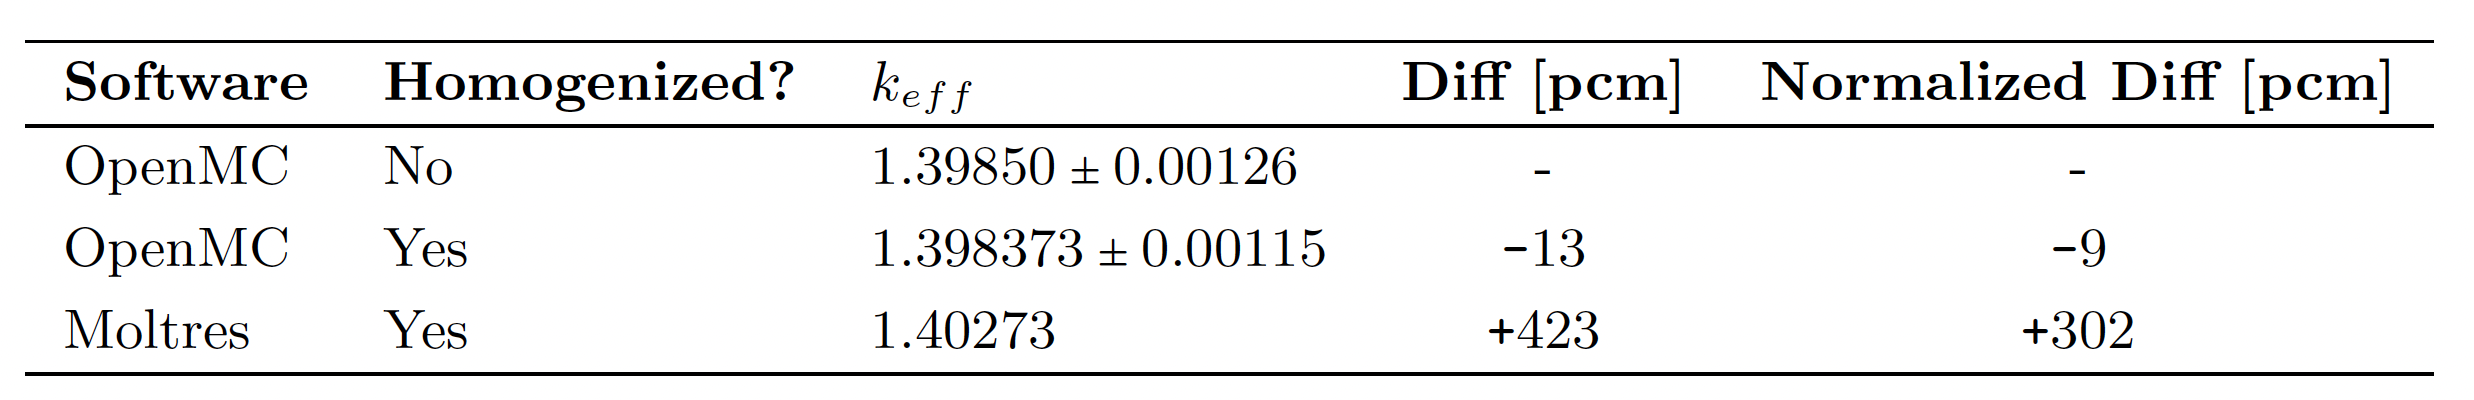
\includegraphics[width=0.9\linewidth]{figures/benchmark-keff.png}
        \end{table}
        The 13pcm $k_{eff}$ and 6pcm reactivity diff, between
        continuous and homogenized OpenMC simulations are within uncertainty, showing 
        that \textbf{selected spatial homogenizations and energy discretizations are 
        acceptable.}
        The Moltres simulation shows a 423pcm diff in $k_{eff}$ and 216pcm 
        diff in reactivity.
        \begin{table}
            \caption{Reactivity coefficients comparison.}
            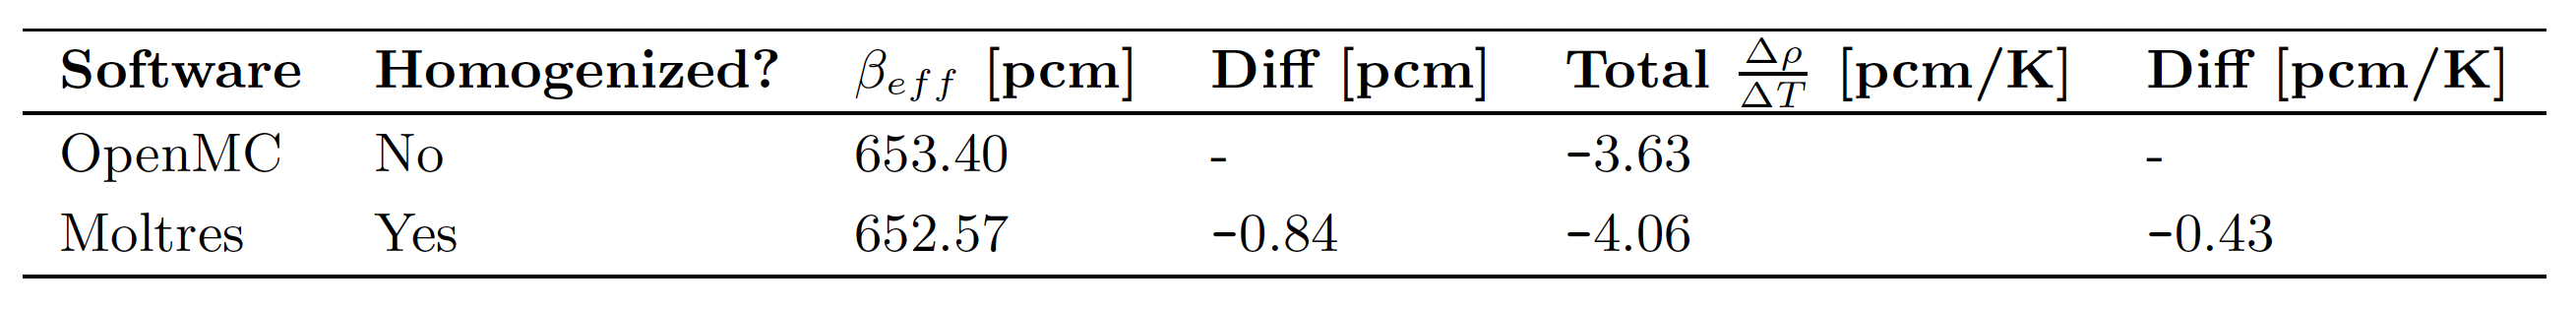
\includegraphics[width=0.85\linewidth]{figures/benchmark-coeff.png}
        \end{table}
        \textbf{Good agreement} for Moltres' delayed neutron fraction ($\beta_{eff}$) and 
        temperature reactivity feedback ($\frac{\Delta \rho}{\Delta T}$)
\end{frame}

\begin{frame}
    \frametitle{AHTR Temp Model Flux Verification}
    \begin{columns}
    \begin{column}{0.7\textwidth}
    \begin{figure}[]
        \centering
        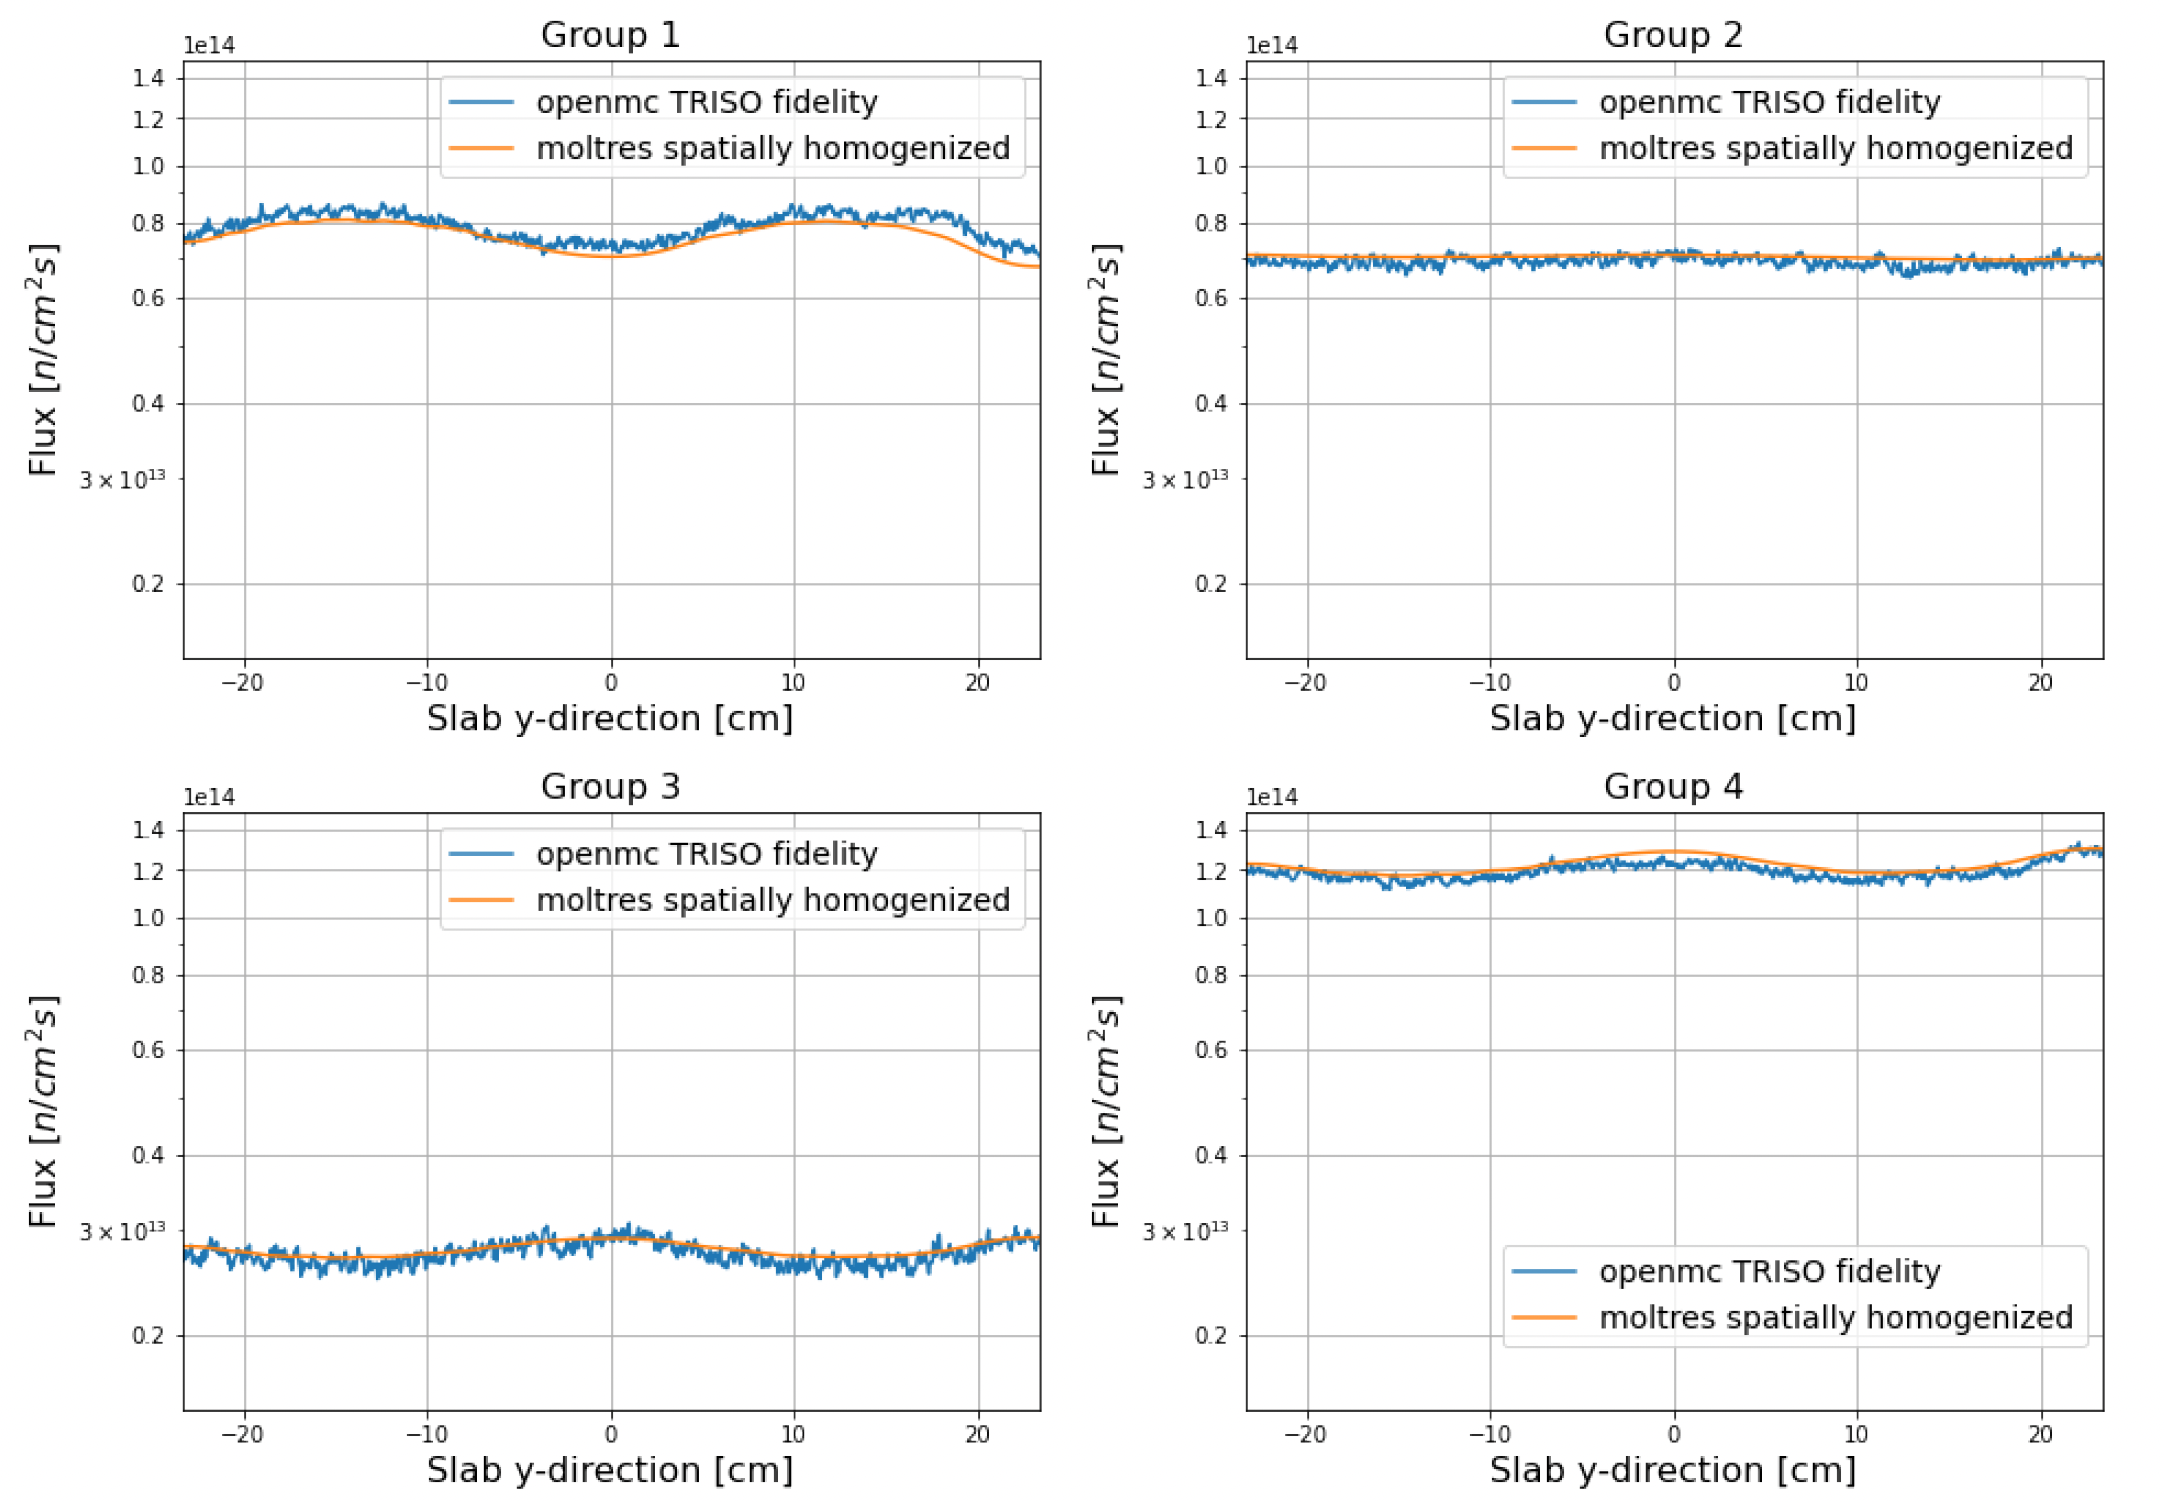
\includegraphics[width=\linewidth]{figures/benchmark-flux.png} 
        \caption{4-group flux distribution comparison.}
    \end{figure}
    \end{column}
    \begin{column}{0.3\textwidth}
        2-norm Diff [\%]
        \begin{itemize}
            \item Group 1: 0.13\% 
            \item Group 2: 0.08\% 
            \item Group 3: 0.10\% 
            \item Group 4: 0.09\%
        \end{itemize}
        Max Diff [\%]
        \begin{itemize}
            \item Group 1: -10.57\% 
            \item Group 2: +7.58\% 
            \item Group 3: +8.96\% 
            \item Group 4: +6.97\%
        \end{itemize}
    \end{column}
    \end{columns}
\end{frame}

\begin{frame}
    \frametitle{AHTR Temp Model Neutron Energy Spectrum Verification}
            \begin{figure}[]
                \centering
                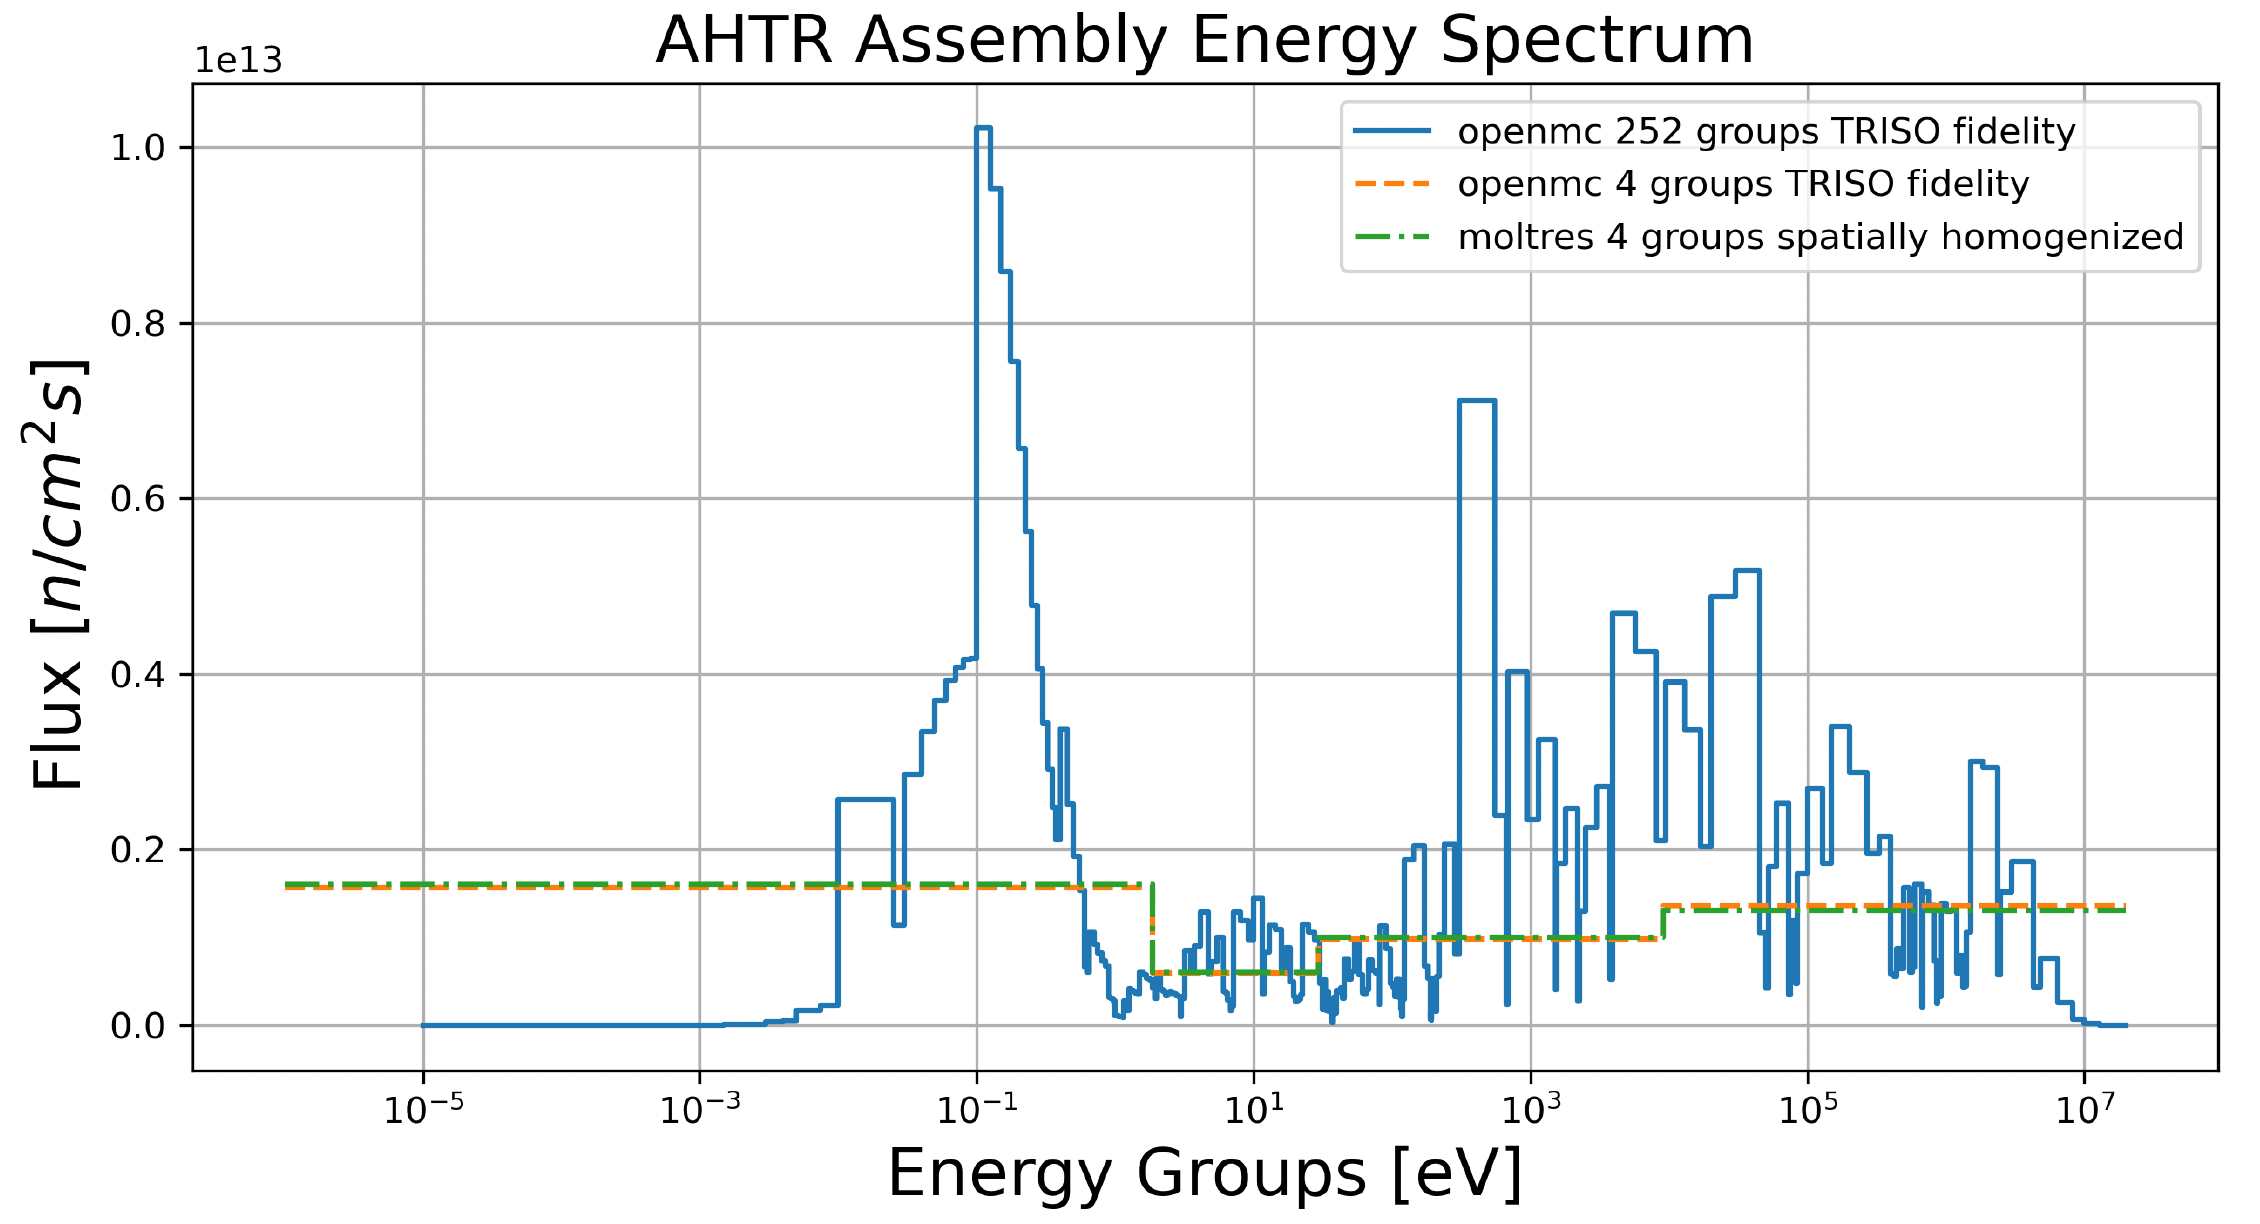
\includegraphics[width=0.75\linewidth]{figures/benchmark-spectrum.png} 
                \caption{Neutron Energy Spectrum Comparison.}
            \end{figure}
        \textbf{Good agreement} between OpenMC and Moltres models 4-group spectrums.
\end{frame}

\begin{frame}
    \frametitle{Key Neutronics Parameter Verification Summary}
    OpenMC vs Moltres models key observations 
    \begin{itemize}
        \item 216 pcm reactivity diff 
        \item Good agreement in reactivity coeffcients and 4-group neutron spectrum
        \item Good agreement in overall flux but larger flux diffs at specific points.
    \end{itemize}
    Explanations 
    \begin{itemize}
        \item Reactivity and flux differences due to Moltres' neutron diffusion method 
        \item Differences in reactivity and flux at specific points might result in 
        slightly inaccurate temperatures at certain points.
        \item Since the reactivity coefficients and overall flux distribution 
        are in agreement, OpenMC's group constants are sufficiently accurate to calculate
        and gain an overall perspective of the AHTR's temperature distribution
    \end{itemize}
    Methodology 
    \begin{itemize}
        \item I use this same Moltres model verification method for the AHTR geometries 
        used for optimization 
    \end{itemize}
\end{frame}

\subsection{AHTR Temperature Model Results}
\begin{frame}
    \frametitle{AHTR Temperature Model Results}
    \begin{columns}
        \begin{column}{0.6\textwidth}
            \begin{figure}[]
                \centering
                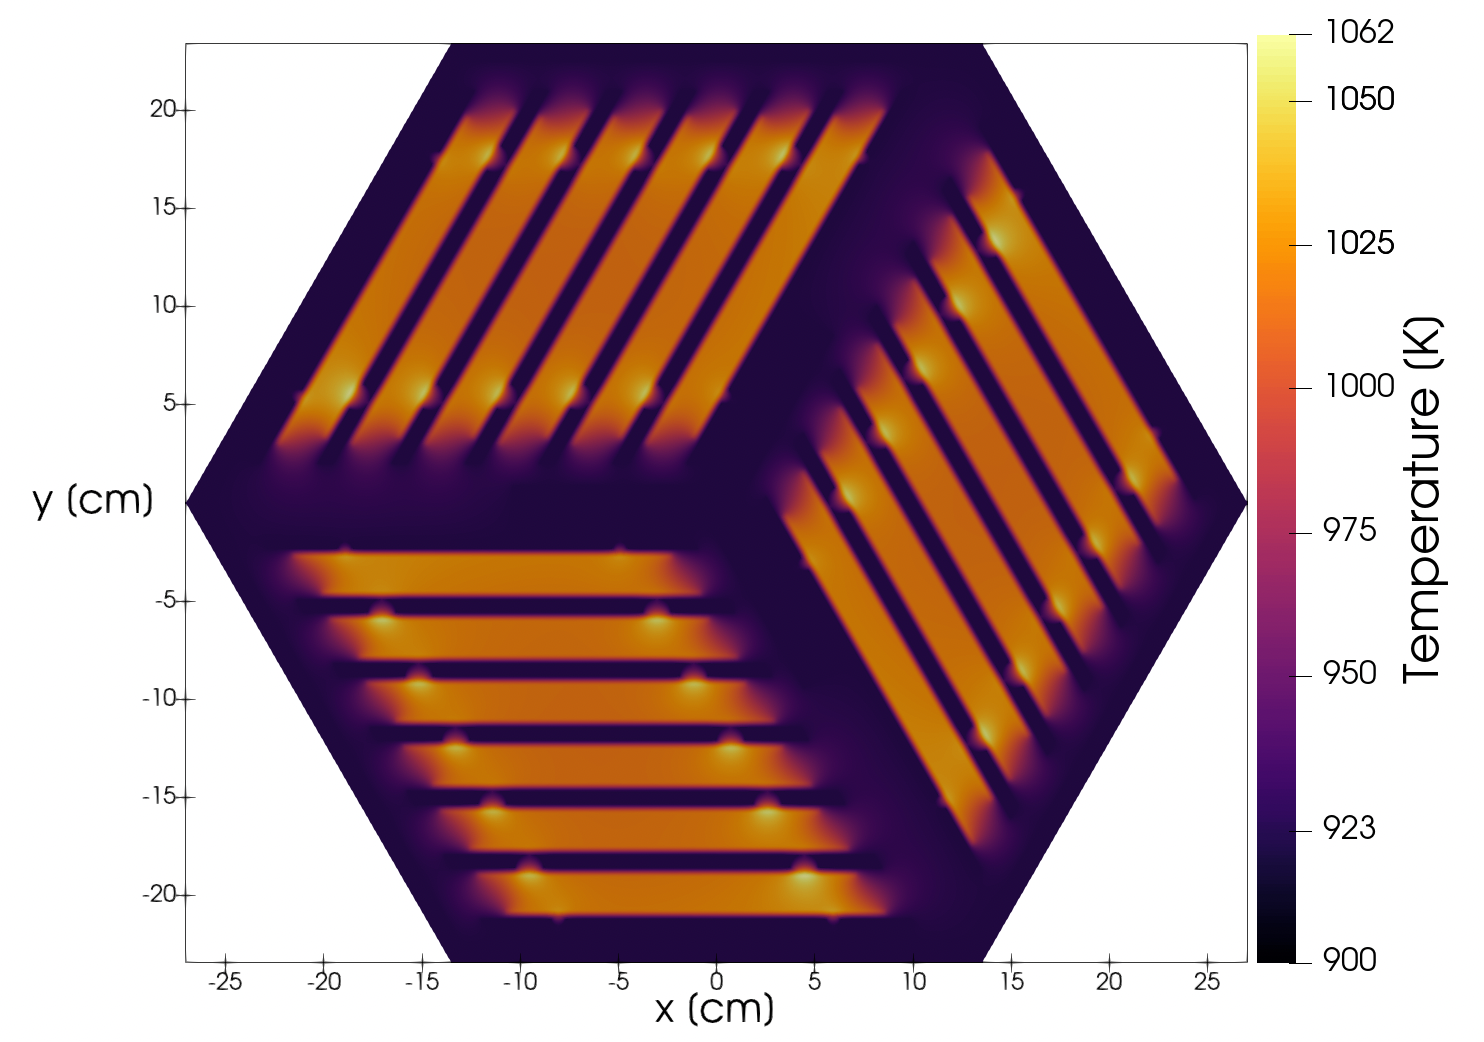
\includegraphics[width=\linewidth]{../docs/figures/benchmark-temperature-model.png} 
                \caption{2D temperature distribution in the \acrfull{AHTR}
                full assembly generated by Moltres.}
            \end{figure}
        \end{column}
        \begin{column}{0.4\textwidth} 
            \begin{block}{Results}
                \begin{itemize}
                    \item Average temperature distribution across the fuel planks are 
                    $\sim 1025K$
                    \item Average temperature of graphite structure is $\sim 935K$
                    \item Temperature peaks at 1062K in the fuel stripes near the spacers
                    \item This could be due to the extra moderation provided by the
                    graphite spacers
                \end{itemize}
            \end{block}
        \end{column}
        \end{columns}
\end{frame}

\subsection{FHR Benchmark + AHTR Model Development: Summary}
\begin{frame}
    \frametitle{FHR Benchmark + AHTR Model Development: Summary}
    \begin{block}{Major Takeaways}
        \begin{itemize}
            \item AHTR has passive safety behavior with negative temperature coeffcients
            \item Increased fuel packing does not always correspond with increased 
            $k_{eff}$ due to self-shielding effects 
            \item These results hint at the possibility of minimizing fuel required by 
            optimizing for heterogenous fuel distributions within the core
            \item AHTR temperature peaks in the fuel stripes near the spacers 
        \end{itemize}
    \end{block}
    \begin{block}{I Successfully Completed AHTR Model Development Research Objectives}
        \begin{itemize}
            \item I furthered our understanding of the AHTR design's complexities 
            through neutronics and multiphysics modeling
            \item I participated in the OECD-NEA's FHR Benchmark Phases I-A and I-B
        \end{itemize}
    \end{block}
\end{frame}
